\chapter{Grundlagen}

\section{Was ist Pfadplanung?}
%SOME OF the most significant challenges confronting autonomous robotics lie in the
%area of automatic motion planning. The goal is to be able to specify a task in a highlevel
%language and have the robot automatically compile this specification into a set of
%low-level motion primitives, or feedback controllers, to accomplish the task. The prototypical
%task is to find a path for a robot, whether it is a robot arm, a mobile robot, or a
%magically free-flying piano, from one configuration to another while avoiding obstacles.
%Proper work
%%(S.1)
%Path planning means to find a collisionfree path for a robot to move from one configuration to another \cite[~S. 1]{Principles:05}. This of course has several constraints given that a robot exists in the real world with physical constraints and limited movement options. 
%(S.1)
Pfadplanung ist die Spezifizierung einer Aufgabe in einer Hochsprache, die ein Roboter verstehen und ausführen soll. Typischerweise ist ein kollisionsfreier Weg zu finden, auf dem sich ein Roboter von einem Punkt zu einem anderen bewegen kann \cite[~S. 1]{Principles:05}. Der Roboter soll die Umgebung wahrnehmen, um sie zu verstehen und erkunden zu können. Außerdem müssen seine Bewegungseinschränkungen betrachten werden, um gültige Pfade zu finden. Deshalb wird die Umgebung in einer für den Roboter verständlichen Sprache dargestellt, die seine Bewegungsoptionen kennt. In diesem Kapitel werden drei Optionen für die Darstellung des Raumes beschrieben: Potentialfeld, Roadmap und Zelldekomposition.
%\\\\
%Pfadplanung kann auch in anderen Bereichen genutzt werden. Beispielsweise in selbstfahrenden Fahrzeugen und Videospielen. 
%Mention more Fields


\section{Konfigurationsraum und freier Raum}\label{Kapitel 2.2}
%\cite{Principles:05}
%TO CREATE motion plans for robots, we must be able to specify the position of the
%robot. More specifically, we must be able to give a specification of the location of
%every point on the robot, since we need to ensure that no point on the robot collides
%with an obstacle. (S. 39)
%
%(S. 40)
%The configuration of a robot system is a complete specification of the position of every
%point of that system. The configuration space, or C-space, of the robot system is the
%space of all possible configurations of the system. Thus a configuration is simply a
%point in this abstract configuration space.
%
%A simple way to represent the robot?s configuration is
%to specify the location of its center, (x, y), relative to some fixed coordinate frame.
%If we know the radius r of the robot, we can easily determine from the configuration
%q = (x, y) the set of points occupied by the robot. We will use the notation R(q) to
%denote this set. When we define the configuration as q = (x, y), we have
%R(x, y) = {(x, y) | (x ? x)2 + (y ? y)2 ? r 2},
%and we see that these two parameters, x and y, are sufficient to completely determine
%the configuration of the circular robot.
%
%Robots move in a two- or three-dimensional Euclidean ambient space, represented
%by R2 or R3, respectively.We sometimes refer to this ambient space as the workspace.
%
%(S. 43)
%We define a configuration space obstacleQOi to be the set of
%configurations at which the robot intersects an obstacle WOi in the workspace,
%
%The free space or free configuration space Qfree is the set of configurations at which
%the robot does not intersect any obstacle, i.e.,
%
%free path = do not touch obstacles
%semifree path = touch obstacles
%
%%Beispiel for workspace (S. 41)
%We define the workspace of the two-joint manipulator to be the reachable points
%by the end effector. The workspace for our two-joint manipulator is an annulus
%(figure 3.3), which is a subset of R2. All points in the interior of the annulus are
%reachable in two ways, with the arm in a right-arm and a left-arm configuration,
%sometimes called elbow-up and elbow-down. Therefore, the position of the end effector
%is not a valid configuration (not a complete description of the location of all points
%of the robot), so the annulus is not a configuration space for this robot.
%Bild (S. 42)
%
%Proper work
%In order to move a robot it's necessary to know the points of the robot that will be moved in order to ensure that no point collides with any obstacles. Therefore the configuration of a robot system is defined as a complete specification of the position of every one of its points. The configuration space of the robot system is the space of all possible configurations of the robot. The workspace can be defined as a two- or three-dimensional Euclidean ambient space in which they move, represented by A and B respectively. 
%
%In the configuration space, an obstacle is defined as the set of configurations at which the robot intersects an obstacle in the workspace. Conversely, the free space or free configuration space is the set of configurations at which the robot does not intersect any obstacle.
%
%The obstacle space of a robot is the configurations of a robot, where he collides with an obstacle
%
%(S. 40, 43)
Das Buch \cite{Principles:05} bietet einige wichtige Definitionen für Pfadplanung. Ein Roboter befindet sich in einer zwei- oder dreidimensionalen euklidischen Umgebung\footnote{Koordinatenraum}, die durch $\mathbb{R}^{2}$ bzw. $\mathbb{R}^{3}$ dargestellt ist. Dies wird als der Arbeitsraum definiert. Für seine Bewegung ist es notwendig, die Position des Roboters im Arbeitsraum zu kennen. Die Positionskoordinaten werden genutzt, um Kollisionen mit Hindernissen zu vermeiden. Daher wird die Konfiguration eines Roboters, als eine vollständige Spezifikation der Position jedes einzelnen seiner Teile definiert. Folglich ist der Konfigurationsraum des Roboters, der Raum aller möglichen Konfigurationen. Dies wir genutzt, um den Roboter zu bewegen, indem er von einer Konfiguration zu einer anderen wechselt.\\
% Beispiel? 
%(S. 43)
% Fussnote ?
Die Konfigurationen, in denen der Roboter ein \textit{Hindernis im Arbeitsraum} schneidet, erzeugen Kollisionen. Der Satz dieser Konfigurationen ist ein \textit{Hindernis im Konfigurationsraum}. 
%Ein Hindernis im Konfigurationsraum wird als Satz von Konfigurationen dargestellt, bei denen der Roboter dieses Hindernis im Arbeitsraum schneidet. 
Umgekehrt ist der freie Raum, oder freie Konfigurationsraum, die Gruppe von Konfigurationen, in denen der Roboter mit keinem Hindernis kollidiert.
% Mention Obstacle space?


\section{Aufgaben} \label{AufgabenPP}
%(9, 10)
%The most important characterization of a motion planner is according to the problem
%it solves. This book considers four tasks: navigation, coverage, localization, and
%mapping. Navigation is the problem of finding a collision-free motion for the robot
%system from one configuration (or state) to another. The robot could be a robot arm,
%a mobile robot, or something else. Coverage is the problem of passing a sensor or
%tool over all points in a space, such as in demining or painting. Localization is the
%problem of using a map to interpret sensor data to determine the configuration of the
%robot. Mapping is the problem of exploring and sensing an unknown environment
%to construct a representation that is useful for navigation, coverage, or localization.
%Localization and mapping can be combined, as in SLAM.
%There are a number of interesting motion planning tasks not covered in detail in this
%book, such as navigation among moving obstacles, manipulation and grasp planning,
%assembly planning, and coordination of multiple robots. Nonetheless, algorithms in
%this book can be adapted to those problems.

%Proper work
Bei der Pfadplanung werden verschiedenen Aufgaben gelöst. Ein Roboter kann eine oder mehrere Aufgaben lösen. Manche Aufgaben sind nach \cite[~S. 9,10]{Principles:05}:
%Die Aufgaben für Pfadplanung sind vielfältig und ein Roboter kann mehrere davon ausführen. Einige Aufgabenbeispiele sind \cite[~S. 9,10]{Principles:05}:
\begin{itemize}
	\item \textit{Navigation} ist die kollisionsfreie Pfadfindung. Sie kann mit stationären und/oder beweglichen Hindernissen durchgeführt werden.
	\item \textit{Lokalisierung} ist die Interpretation von Sensordaten zur Bestimmung der Konfiguration des Roboters.
	\item \textit{Bedeckung\footnote{Bedeckung (engl. Coverage)}} bedeutet das Besuchen von Benutzerdefinierten Punkten des Konfigurationsraums.
	\item \textit{Kartographie} ist die Exploration einer unbekannten Umgebung, um eine aussagekräftige Darstellung davon zu erzeugen.
\end{itemize}

\section{Umgebungsdarstellung}

\subsection{Potentialfunktion und Potentialfeld}
%(S. 77, 78)
%A potential function is a differentiable real-valued function $U : \mathbb{R}^{n} \rightarrow \mathbb{R}$. The value
%of a potential function can be viewed as energy and hence the gradient of the potential
%is force. The gradient is a vector which points in the direction that locally maximally increases U. See appendix C.5 for a
%more rigorous definition of the gradient. We use the gradient to define a vector field,
%which assigns a vector to each point on a manifold. A gradient vector field, as its name
%suggests, assigns the gradient of some function to each point. When U is energy, the
%gradient vector field has the property that work done along any closed path is zero.
%The potential function approach directs a robot as if it were a particle moving
%in a gradient vector field. Gradients can be intuitively viewed as forces acting on a
%positively charged particle robot which is attracted to the negatively charged goal.
%Obstacles also have a positive charge which forms a repulsive force directing the robot
%away from obstacles. The combination of repulsive and attractive forces hopefully
%directs the robot from the start location to the goal location while avoiding obstacles
%(figure 4.1).
%Potential functions can be viewed as a landscape where the robots move from a
%?high-value? state to a ?low-value? state. The robot follows a path ?downhill? by
%following the negated gradient of the potential function. Following such a path is
%called gradient descent, i.e.,
%
%%Gradient (483)
%Von \cite[~S. 483]{Principles:05}: Gegeben die Funktion $g : \mathbb{R}^{n} \rightarrow \mathbb{R}$, die Gradient von \textit{g} ist definiert als:
%$$
%\nabla g =
%\begin{bmatrix}
%frac{\partial g}{
%\partial x1}
%frac{\partial g}{
%\partial x2}
%...
%frac{\partial g}{
%\partial xn}
%\end{bmatrix}
%$$
%%(A Potential Field Approach to Path Planning) \cite{Yong:92}
%In the potential field approach, obstacles are assumed to
%carry electric charges, and the resulting scalar potential field
%is used to represent the free space. Collisions between the obstacles
%and the robot are avoided by a repulsive force between
%them, which is simply the negative gradient of the potential
%field.
%%Proper Work
%%(77,78)
%A potential function is a differentiable function $U : \mathbb{R}^{n} \rightarrow \mathbb{R}$, which can be viewed as energy. Its gradient is a vector which points in the direction that locally maximally increases U. (Definition gradient) By assigning a gradient to each point of a vector field, a potential field is created. 
%In order to move the robot along said field, it is treated as a particle with a positive charge. The obstacle are positively charge, causing them to repel each other, and the goal is negatively charged, causing it to move towards it. This means the robot follows a path ?downhill? by following the negated gradient of the potential function.
%Bild
% Sein Gradient ist ein Vektos .... -> Verbessern
%Sein Gradient ist ein Vektor, der in die Richtung zeigt, in der $U$ lokal maximal zunimmt.
Laut \cite{Principles:05} ist eine Potentialfunktion eine differenzierbare Funktion $U : \mathbb{R}^{n} \rightarrow \mathbb{R}$, die als Energie betrachtet werden kann. Ihr Gradient ist ein Vektor, welcher das Verhalten der Funktion beschreibt. Er zeigt in die Richtung, in der $U$ lokal maximal zunimmt. Indem jedem Punkt eines Konfigurationsraum ein Gradient zugeordnet wird, entsteht ein Potentialfeld.\\
Um den Roboter entlang dieses Feldes zu bewegen, wird er wie ein Teilchen mit einer positiven Ladung besetzt. Die Hindernisse sind positiv geladen, sodass sie und der Roboter sich gegenseitig abstoßen. Das Ziel ist negativ geladen, sodass der Roboter sich darauf zubewegt. Deshalb wird ein absteigender Weg durchgelaufen. Abbildung \ref*{potentialfield01} zeigt ein Potentialfeld mit zwei Hindernissen.
% indem der Roboter dem negativen Gradienten der Potentialfunktion folgt.
%Bild?
\begin{figure}[H] %Von Website
	\centering
	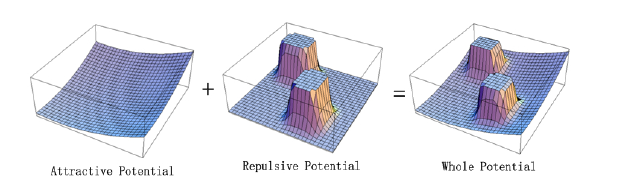
\includegraphics[width=0.8\textwidth]{images/Potential_Field.png}
	\caption{Abb. 3.7 von \cite{Petersen:15}: Bildliche Erläuterung der Potentialfeldmethode. Links: Anziehendes Potential des Ziels, Mitte: Abstoßendes Potential der Hindernisse, Rechts: Kombination bzw. entstandenes Potentialfeld.}
	\label{potentialfield01}
\end{figure}


\subsection{Roadmaps}
%(S. 107)
%If we knew that many paths were to
%be planned in the same environment, then it would make sense to construct a data
%structure once and then use that data structure to plan subsequent paths more quickly.
%This data structure is often called a map, and mapping is the task of generating models
%of robot environments from sensor data.
%(107 - 108)
%In the context of indoor systems, three
%map concepts prevail: topological, geometric, and grids
%%-Topological representations aim at representing environments with graphlike structures,
%%where nodes correspond to ?something distinct? and edges represent an adjacency
%%relationship between nodes.
%%-Geometric models use geometric primitives for representing the environment. Mapping
%%then amounts to estimating the parameters of the primitives to best fit the sensor
%%observations
%%-Finally occupancy grids are grid structures, similar as those described in chapter 4,
%%where the value of each pixel corresponds to the likelihood that its corresponding
%%portion of workspace or configuration space is occupied
%(108)
%This chapter focuses on a class of topological maps called roadmaps [91, 262]. A
%roadmap is embedded in the free space and hence the nodes and edges of a roadmap
%also carry physical meaning. For example, a roadmap node corresponds to a specific
%location and an edge corresponds to a path between neighboring locations. So, in
%addition to being a graph, a roadmap is a collection of one-dimensional manifolds
%that captures the salient topology of the free space.
%(108)
%Likewise, using a roadmap, the planner can construct a path between any two
%points in a connected component of the robot?s free space by first finding a collisionfree
%path onto the roadmap, traversing the roadmap to the vicinity of the goal, and
%then constructing a collision-free path from a point on the roadmap to the goal. The
%bulk of the motion occurs on the roadmap and thus searching does not occur in a
%multidimensional space, whether it be the workspace or the configuration space. If
%the robot knows the roadmap, then it in essence knows the environment. So one way a
%robot can explore an unknown environment is by relying on sensor data to construct a
%roadmap and then using that roadmap to plan future excursions into the environment.
%
%In this chapter, we consider five types of roadmaps: visibility maps, deformation
%retracts, retract-like structures, piecewise retracts and silhouettes.
%Visibility Map Beispiel?
%(S. 12)
%In chapter 5, we introduce more concise representations of the robot?s free space
%that a planner can use to plan paths between two configurations. These structures are
%called roadmaps. A planner can also use a roadmap to explore an unknown space. By
%using sensors to incrementally construct the roadmap, the robot can then use the
%roadmap for future navigation problems.
%
%(110)
%The defining characteristics of a visibility map are that its nodes share an edge if they
%are within line of sight of each other, and that all points in the robot?s free space are
%within line of sight of at least one node on the visibility map. This second statement
%implies that visibility maps, by definition, possess the properties of accessibility
%and departability. Connectivity must then be explicitly proved for each map for the
%structure to be a roadmap. In this section, we consider the simplest visibility map,
%called the visibility graph
%Proper Work
%(12, 107, 108)
%A Robot can use its sensor data in order to connect points in its free space and creating collisonfree paths between them. This creates a topological map, in this case called a roadmap. A planner can use this map in order to explore unknown space by progressively building the roadmap with its sensors.
%The three important steps for a planner to navigate the roadmap are: Finding a road into the roadmap, moving through the roadmap to the vicinity of the goal and finally making a path to the goal.
%(12, 107, 108)
Nach \cite{Principles:05} kann ein Roboter seine Sensordaten verwenden, um Punkte in seinem freien Raum zu verbinden und kollisionsfreie Pfade zwischen ihnen zu erzeugen. Dadurch entsteht eine topologische Karte aus Knoten und Kanten, in diesem Fall eine so genannte Roadmap. Diese Karte kann verwendet werden, um unbekannten Raum zu erkunden, indem er zunehmend die Roadmap mit seinen Sensoren aufbaut.
Die drei Schritte, die Roadmap zu durchlaufen, sind (1) Ein Weg in der Roadmap finden. (2) Durch die Roadmap in die Nähe des Ziels bewegen. (3) Einen Weg zum Ziel finden.
%Formal Definition?
%(109)
%A few types of roadmaps are: visibility maps, deformation retracts, retract-like structures, piecewise retracts and silhouettes.
Ein populärer Typ von Roadmaps ist der Sichtbarkeitsgraph.
%More Info on Visibility Graph?
%Voronoi Diagram?


\subsection{Zelldekomposition}
%(161, 162)
%NEXT, WE consider a different type of representation of the free space called an exact
%cell decomposition. These structures represent the free space by the union of simple
%regions called cells. The shared boundaries of cells often have a physical meaning
%such as a change in the closest obstacle or a change in line of sight to surrounding
%obstacles. Two cells are adjacent if they share a common boundary. An adjacency
%graph, as its name suggests, encodes the adjacency relationships of the cells, where
%a node corresponds to a cell and an edge connects nodes of adjacent cells.
%Assuming the decomposition is computed, path planning with a cell decomposition
%is usually done in two steps: first, the planner determines the cells that contain the start
%and goal, respectively, and then the planner searches for a path within the adjacency
%graph. Note that the adjacency graph could serve as a roadmap of the free space as
%well. Therefore, mapping can be achieved by incrementally constructing the adjacency
%graph.
%Cell decompositions, however, distinguish themselves from other methods in that
%they can be used to achieve coverage. A coverage path planner determines a path
%that passes an effector (e.g., a robot, a detector, etc.) over all points in a free space.
%Since each cell has a simple structure, each cell can be covered with simple motions
%such as back-and-forth farming maneuvers; once the robot visits each cell, coverage
%is achieved. In other words, coverage can be reduced to finding an exhaustive walk
%through the adjacency graph. Sensor-based coverage is achieved by simultaneously
%covering an unknown space and constructing its adjacency graph.
%The most popular cell decomposition is the trapezoidal decomposition [356].
%This decomposition relies heavily on the polygonal representation of the planar
%configuration space. A more general class of decompositions, which are termed
%Morse Decompositions [12], allow for representations of nonpolygonal and nonplanar
%spaces. Morse decompositions are based on ideas from Canny?s roadmap work.
%We then consider a broader class of decompositions which includes those based on
%visibility constraints. One such decomposition serves as a basis for the pursuit/evasion
%problem which is introduced section 6.3.

%Proper work
%Cell decomposition consists of dividing the free space into cells, each division signifying an important change in the space. For Example a change in line of sight to surrounding obstacles. Taking each cell as a node and their shared boundaries as an edge, an adjacency graph can be created.
%Using this graph the path planer follows two steps: determining the start and end nodes, and searching for a path in the adjacency graph.
%A big dvantage they provide is coverage. The graph can be used to visit all points in the free space by exploring the relative simple structure of the cells.
%(161, 162)
In \cite{Principles:05} ist beschrieben, dass Zelldekomposition die Teilung des freien Raumes in Zellen ist, wobei jede Trennung bei einer bemerkenswerten Veränderung des Raumes geschieht. Beispielsweise kann eine Änderung der Sichtlinie zu umgebenden Hindernissen eine Trennung erzeugen. Dadurch ist der komplexere Raum durch weniger komplexe Zellen definiert. Wird jede Zelle als ein Knoten und ihre gemeinsamen Grenzen als eine Kante genommen, kann ein Graph erstellt werden. Der Graph wird Adjazenzgraph genannt, weil er die anliegenden Zellen beschreibt. 
Mit dem Graph kann das Pfadfindungsproblem mit den folgenden Schritten gelöst werden: (1) Bestimmung der Zellen mit der Start- und Endkonfiguration. (2) Suche nach einem Pfad im Adjazenzgraphen.\\
Ein großer Vorteil von Zelldekomposition ist ihre Nutzung für die \textit{Coverage} Aufgabe (\ref{AufgabenPP}). Mit dem Graphen können alle Punkte im freien Raum besucht werden, indem die Zellen erkundet werden.
%Trapezoidal dekomposition

\begin{figure}[H] %Von Website
	\centering
	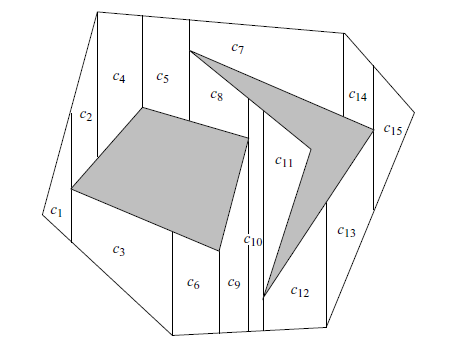
\includegraphics[width=0.7\textwidth]{images/Cell_Dekomposition.png}
	\caption{Schnitt der Abb. 6.2 von \cite{Principles:05}: Teilung eines polygonalen Konfigurationsraums}
	\label{potentialfield02}
\end{figure}

\section{Graphen}
% %Dazu sind Graphen wichtig, weil durch ihre Traversierung einen Pfad gefunden werden kann.
Pfadfindung ist ein Teil der Pfadplanung. Mit Hilfe von Graphen kann ein Pfad gefunden werden. Dazu muss dieser von einem Planer traversiert werden. Laut \cite{Turau:15} bestehen gewichtete Graphen aus Knoten, Kanten und Kosten (siehe \ref{sec0a}). Pfadfindungsalgorithmen nutzen diese Informationen, um sich vom Startknoten bis Endknoten durch die Kanten zu bewegen. Kanten können nur eine Richtung haben, was sie unidirektional statt bidirektional macht. Dies ist hilfreich für die Unterscheidung zwischen ausgehenden und eingehenden Kanten.

\begin{figure} %Von Website
	\centering
	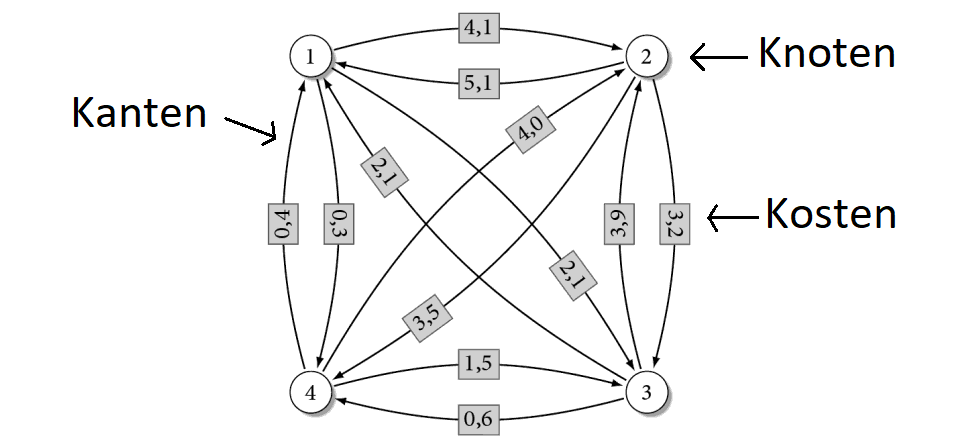
\includegraphics[width=0.9\textwidth]{images/kk_graph_S6.png}
	\caption{Abb. 1.5 von \cite[~S. 6]{Turau:15}. Gewichteter Graph mit Kantenkosten.(gekennzeichnet)}
	\label{sec0a}
\end{figure}

\subsection{Bäume}
Laut \cite{Turau:15} sind Bäume Graphen, die häufig für die Darstellung von hierarchischen Relationen genutzt werden. Ein Baum mit $m$ Knoten hat $m-1$ Kanten.
Gegeben ist ein Baum mit Wurzel $w$. Die Tiefe eines Knotens $e$ ist die Anzahl der Kanten von $w$ nach $e$. Die Wurzel $w$ hat die Tiefe 0. Die Höhe des Baumes ist die maximale Tiefe seiner Knoten.  Der Baum in Abbildung \ref{sec0b} hat die Höhe 3 und die Tiefe des Knotens $e$ beträgt 2.
%ist die Höhe des Baumes 3 und die Tiefe des Knotens $e$ ist 2.

\begin{figure} %Von Website
	\centering
	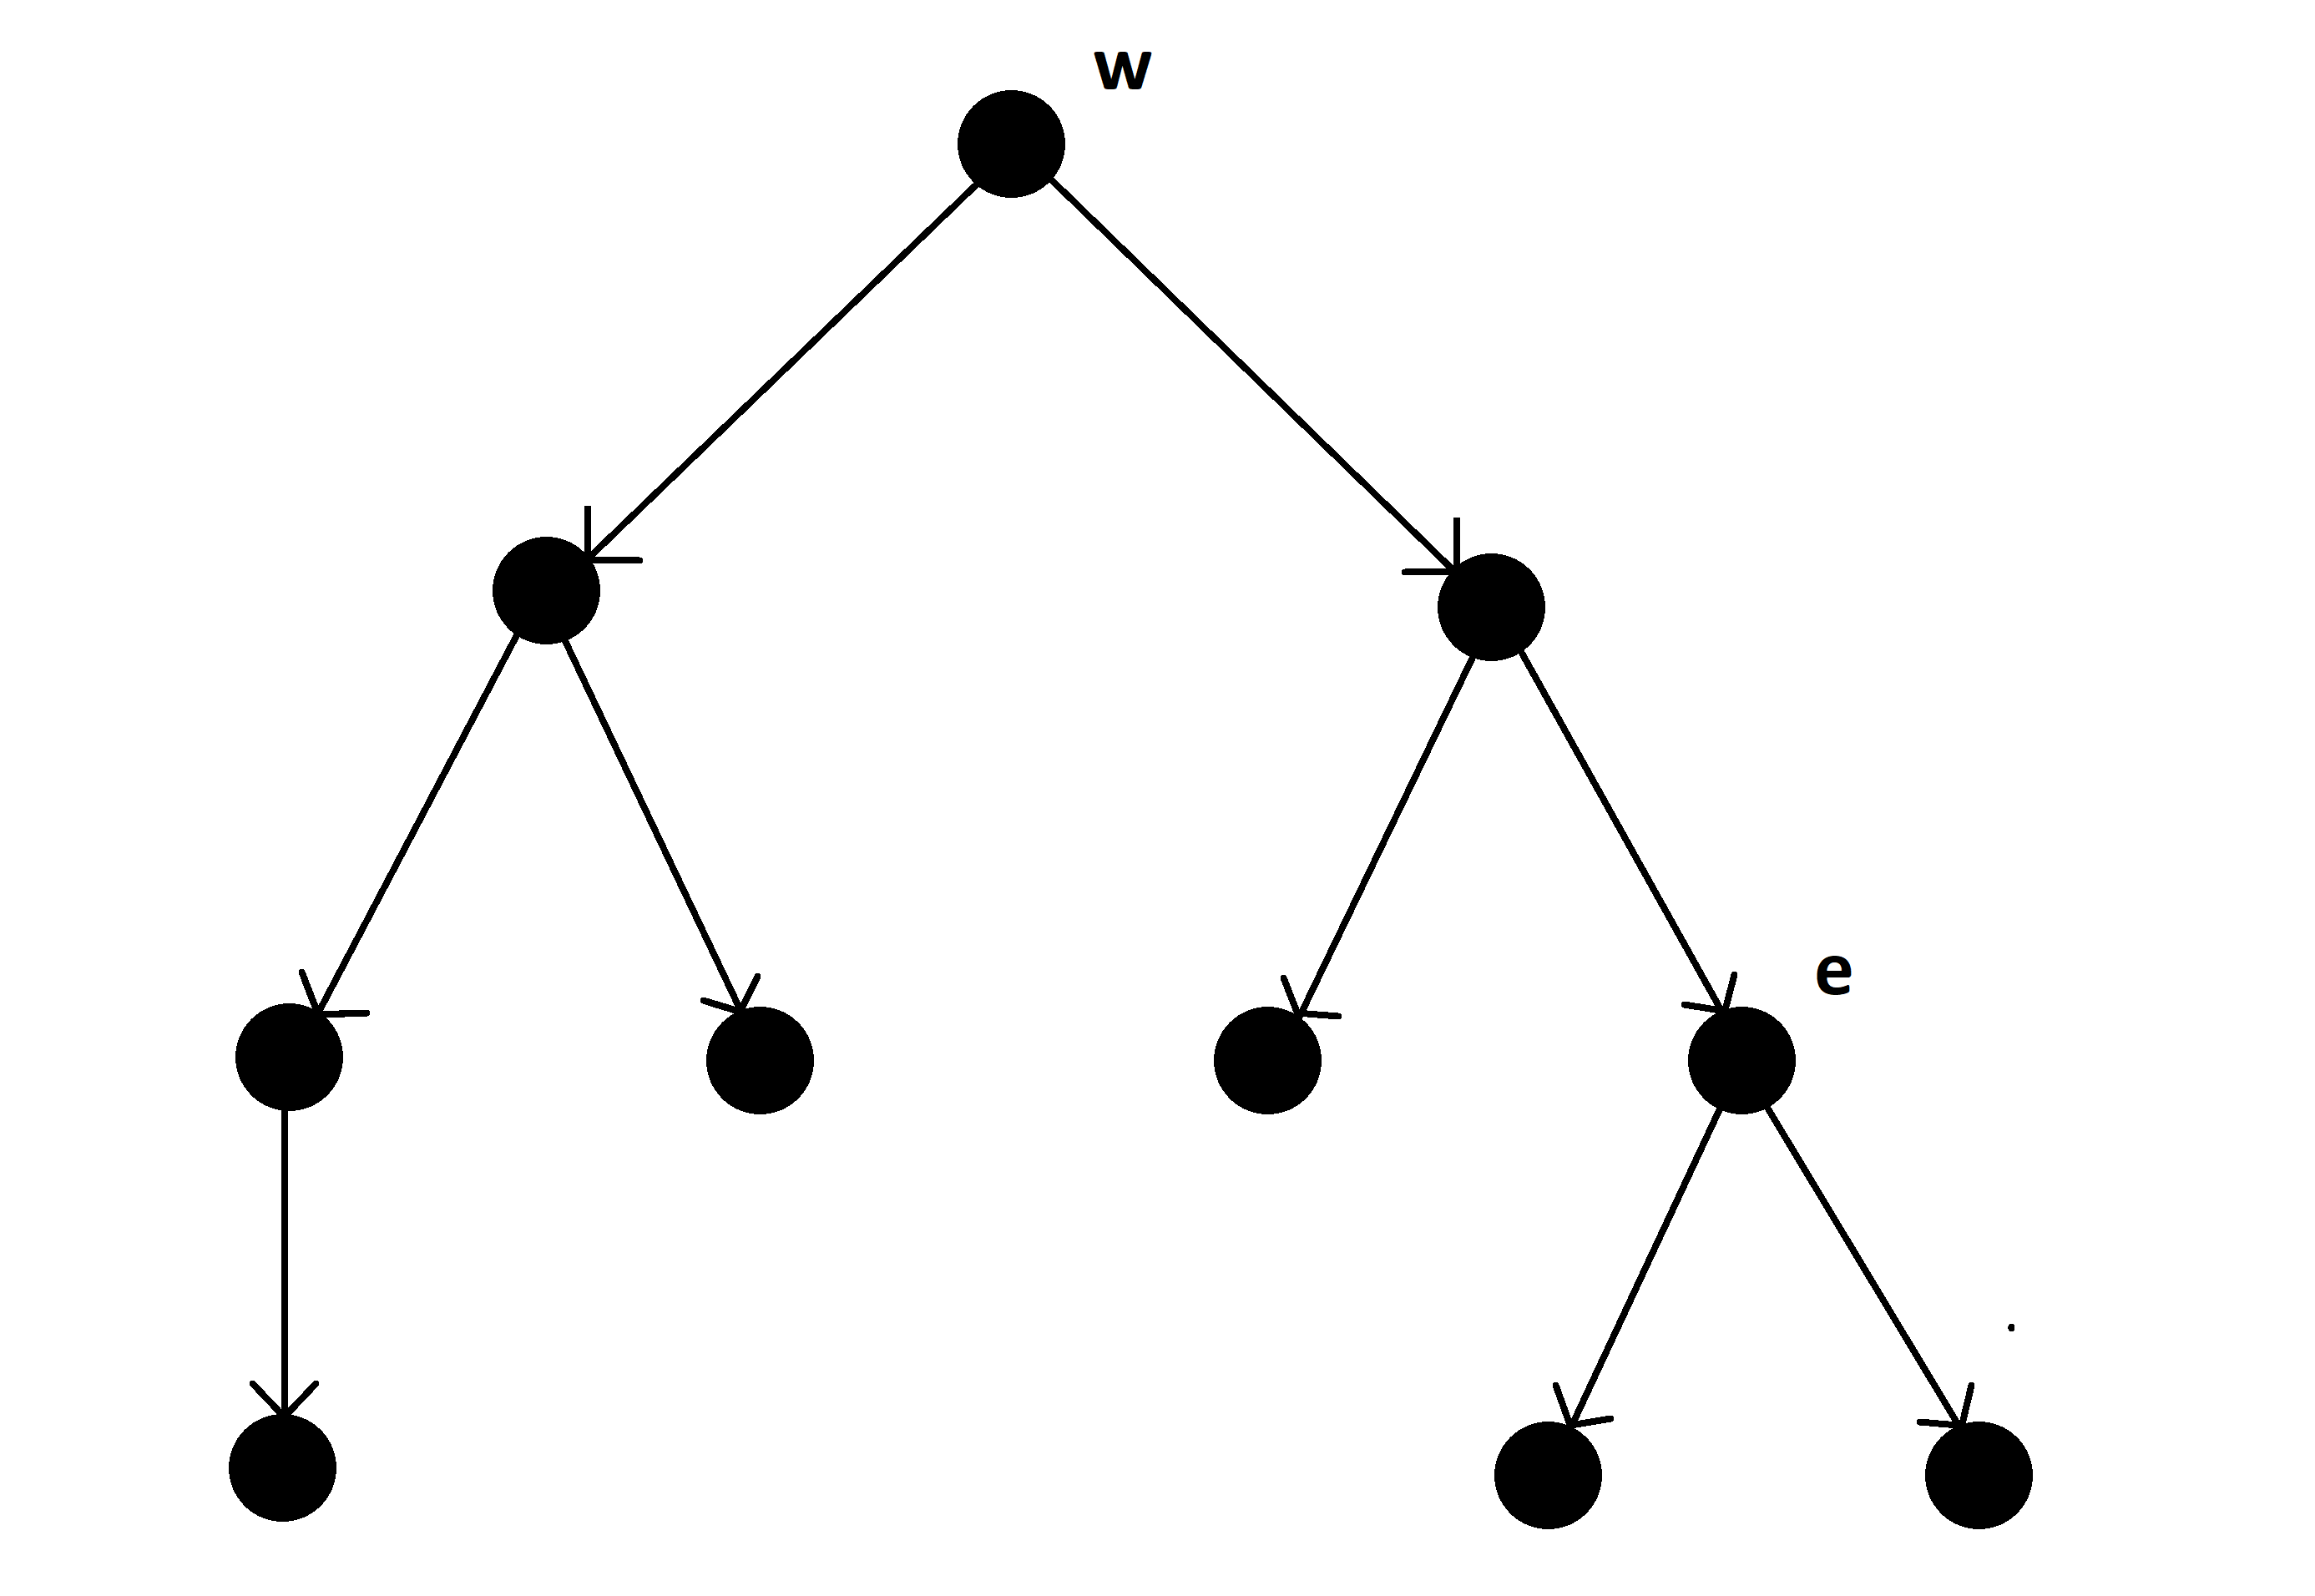
\includegraphics[width=0.5\textwidth]{images/Tree_Graph.png}
	\caption{Ein Baum mit Wurzel $w$}
	\label{sec0b}
\end{figure}

\subsection{Navigationsnetze (\textit{eng.} Navigation Meshes)}
%\cite{Mesh:11}
%A common strategy for efficiently computing realistic
%paths is to partition the environment into a collection of
%walkable areas. This partition is often referred to as a
%navigation mesh. A useful data structure that can be used to
%construct a navigation mesh is the medial axis. The medial
%axis is the set of all points in an environment that have
%more than one distinct closest point on the boundary of the
%environment
%\cite{Mesh:16}
%(91)
%The behavior of characters may also include crawling, running, and other
%surface-based movement, but we will speak of walking and walkable
%surfaces for simplicity. The walkable surfaces of an environment
%form the free space Efree, which is usually less complex than
%the environment itself.
%A navigation mesh is a representation of Efree as a set of (usually
%polygonal) regions, along with a graph that describes how these
%regions are connected.
%(92)
%Let n be the number of vertices required to define Eobs or Efree
%using simple polygons. We call n the complexity of E.
%(93)
%A walkable environment (WE) is a set of interior-disjoint polygons
%in R3 on which characters can stand and walk. Thus, a WE is a
%clean representation of the free space Efree of a 3DE, based on the
%filtering parameters and character properties mentioned earlier. Any
%two polygons are directly connected if and only if characters can
%walk directly between them.
%
%Now that we have a definition of the free space Efree, we can define
%a navigation mesh as a tupleM= (R; G):
% R = fR0;R1; : : :g is a collection of geometric regions in R3
%that represents Efree. Each region Ri is P-simple, by which
%we mean that a region cannot intersect itself when projected
%onto the ground plane P.
% G = (V;E) is an undirected graph that describes how characters
%can navigate between the regions in R.
%Proper Work
%(91,93) \cite{Mesh:16}
%A Navigation mesh is a representation of the free space as polygonal areas alongside a navigation graph that describes how they are connected. The polygonal areas are the regions where an actor can move, refered to as walkable areas. The navigation graph describes how said actor can move to the next area, as in any surface based movement such as walking. As well as providing the requirements for path planning. pathfinding A navigation mesh can be applied to 3D and 2D environments.
%(91,93)
Nach \cite{Mesh:16} ist ein Navigationsnetz die Darstellung des freien Raums, als polygonale Bereiche. Ein Navigationsgraph definiert die Verbindungen zwischen den Gebieten. Die polygonalen Bereiche sind die Regionen, in denen sich ein Akteur bewegen kann. Sie werden als begehbare Flächen\footnote{begehbare Flächen (\textit{eng. walkable areas})} bezeichnet. Der Navigationsgraph beschreibt, wie sich der Akteur zu benachbarten Bereichen bewegen kann. Die Bewegungen sind oberflächenbasiert, beispielsweise Gehen oder Rennen. Ein Navigationsnetz kann sowohl auf 3D- als auch auf 2D-Umgebungen angewandt werden.

\begin{figure}[H] %Von Website
	\centering
	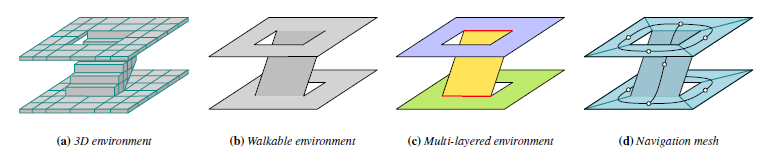
\includegraphics[width=\textwidth]{images/navigation_mesh_16.png}
	\caption{Von \cite[~S. 93]{Mesh:16} \textit{Abb. 2}. Verschiedene Darstellungen einer Umgebung und ein Beispiel für ihr Navigationsnetz. (a) Eine 3D-Umgebung besteht aus unbearbeiteter 3D-Geometrie. (b) Der freie Raum einer 3D-Umgebung. Eine begehbare Umgebung enthält nur begehbare Oberflächen. (c) Eine mehrschichtige Umgebung, ist in Schichten unterteilt. (d) Ein Navigationsnetz ist die Beschreibung einer begehbaren Umgebung für Pfadplanungszwecke.}
	\label{sec1a}
\end{figure}
\begin{figure}[H] %Von Website
	\centering
	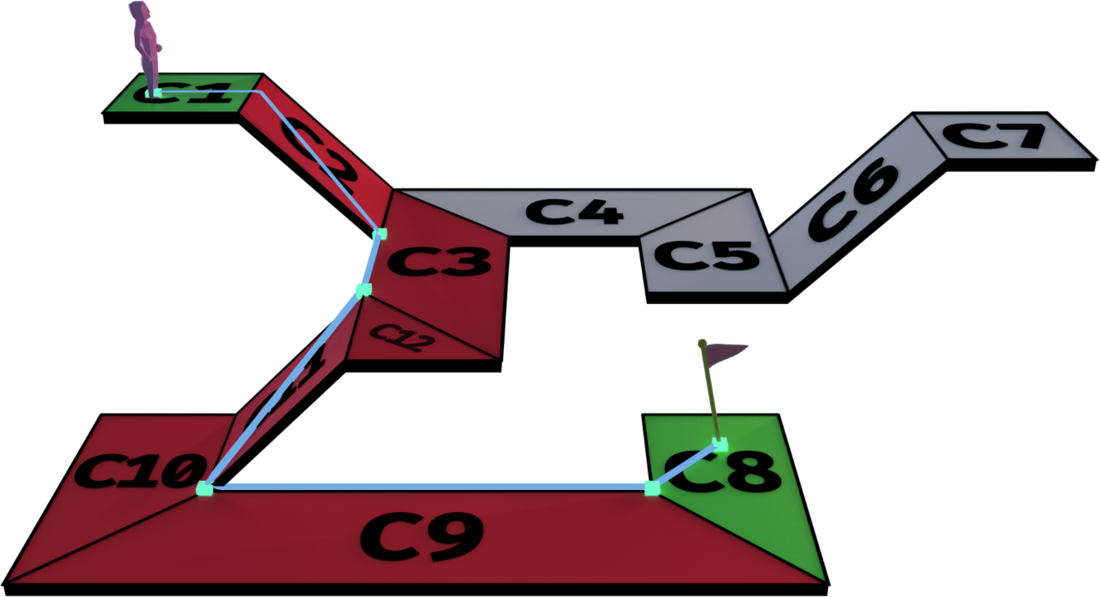
\includegraphics[width=0.6\textwidth]{images/mesh_with_path.png}
	\caption{Von \cite{Mesh:18}: Navigation Mesh mit einem Pfad von Startpunkt C1 bis Endpunkt C8.}
	\label{sec1b}
\end{figure}


\subsection{Rastergraph (\textit{eng.} Grid Graph)}
%A Star is good for them
%Grids are composed of tiles which lie adjacent to each other
%A raster is put on top of the environment where it will be used. Then a Graph Search with its Tiles is used to find a path in it. For that each Tile possess a travel cost. A common Pathfinding Algorthim used here is A*.
%A common Tile has 4 adjacent Tiles, however more options for a grid are possible. A hextile has six neighbours and the Octile has eight, 4 adjacent like the regular tile and 4 from diagonal movement.
%(1) Raster bestehen aus Felder, die nebeneinander liegen.
Raster werden aus einem Netz von zusammenhängenden Feldern gebildet.
Laut \cite{Grid:02} wird ein Raster über die Umgebung gelegt, in der es genutzt wird.
Wenn die Felder als Knoten betrachten werden, kann eine Graphensuche verwendet werden, um einen Pfad darin zu finden.
Dafür besitzt jedes Feld Kanten zu seinen Nachbarn. 
Ein üblicher Pfadfindungsalgorithmus dafür ist A*.
\\
Felder können unterschiedlich viele Nachbarn besitzen.
Rechteckige Felder haben vier benachbarte Felder.
Ein sechseckiges Feld hat sechs Nachbarn. Wenn die Diagonalen betrachtet werden, haben die rechteckigen Felder acht Nachbarn (siehe Abbildung \ref{sec2a}).
%Für den Graph hat eine Feld typischerweise vier benachbarte Felder, es sind jedoch mehr Optionen möglich. Eine sechseckige Feld hat sechs Nachbarn und die normale rechteckige Feld hat dann acht, wenn die Diagonalen betrachtet werden (siehe Abb. \ref{sec2a}).
\begin{figure} %Gemacht mit Paint
	\centering
	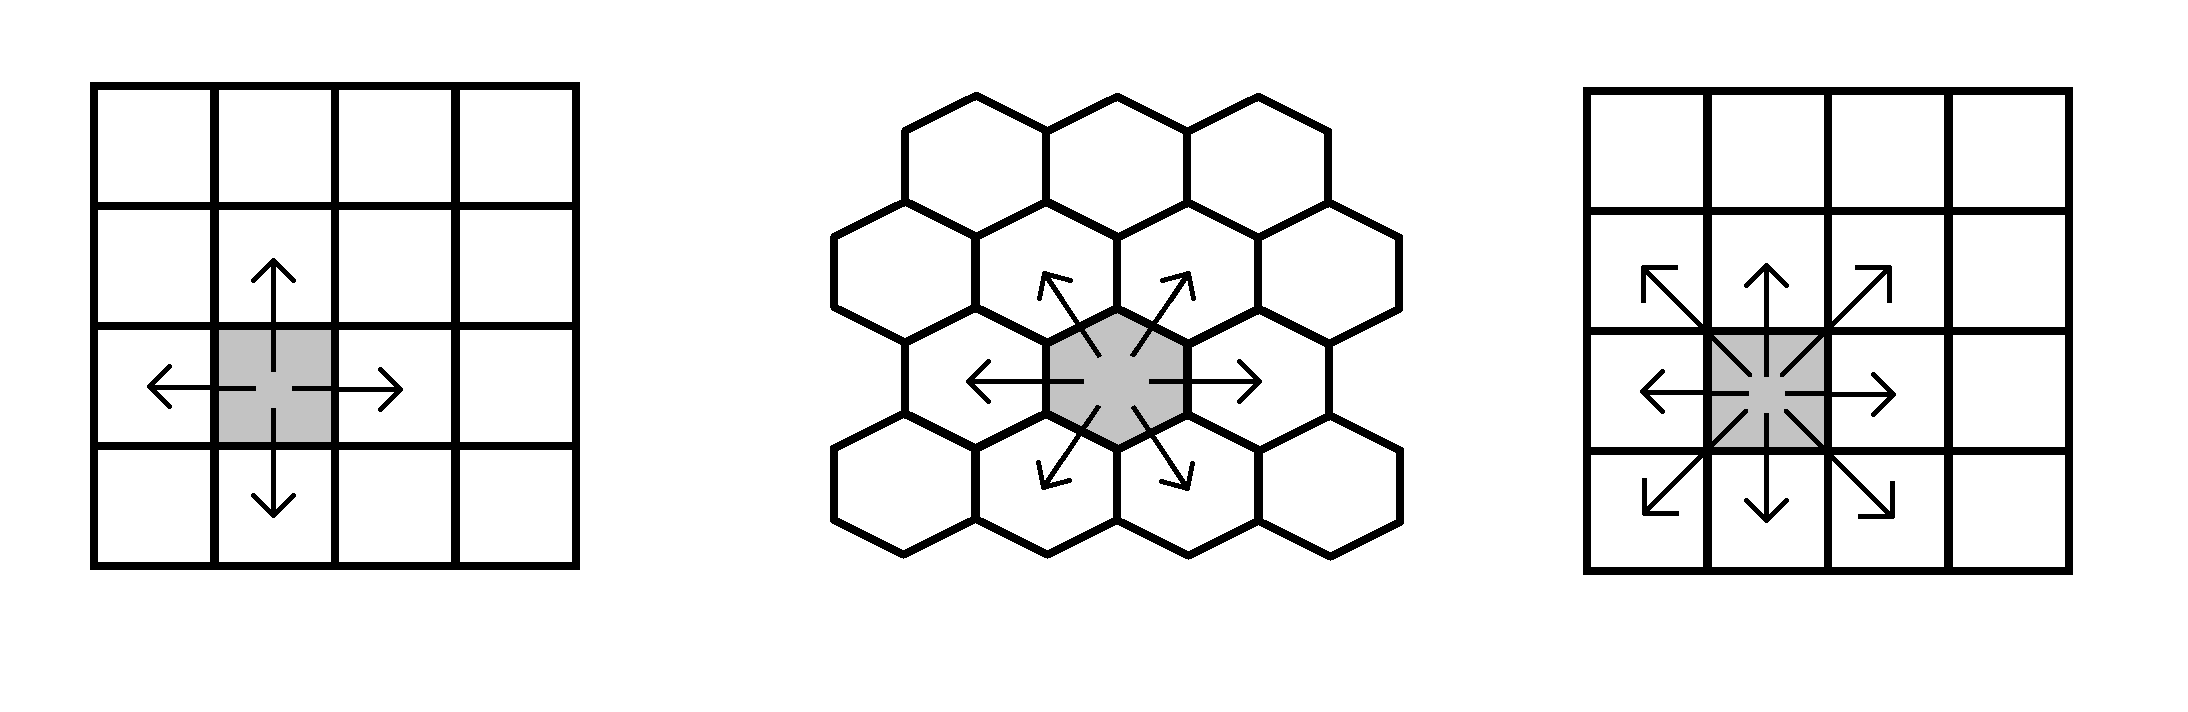
\includegraphics[width=\textwidth]{images/Grid_Tiles.png}
	\caption{Von links nach rechts: Feld mit 4 Bewegungsoptionen, Hexagon mit 6 Bewegungsoptionen, Feld mit 8 Bewegungsoptionen.}
	\label{sec2a}
\end{figure}


\subsection{Sichtbarkeitsgraph (\textit{eng.} Visibility Graph)}
%(110)
%The defining characteristics of a visibility map are that its nodes share an edge if they
%are within line of sight of each other, and that all points in the robot’s free space are
%within line of sight of at least one node on the visibility map.
%
%The standard visibility graph is defined in a two-dimensional polygonal configuration
%space (figure 5.3). The nodes vi of the visibility graph include the start location,
%the goal location, and all the vertices of the configuration space obstacles. The graph
%edges ei j are straight-line segments that connect two line-of-sight nodes vi and vj , i.e.,
%Proper Work
%(110)
%Visibility graphs consist of nodes that share an edge if they are withhin line if sight with each other and no obstacle lies between them. The standard Graph is two dimensional. Possesing the start point, end point and the vertices of the polygons that represent obstacles as nodes.
%
%An example of a visibility graph lies in image ref.
%(110)
%In \cite{Principles:05} ist beschrieben, dass Sichtbarkeitsgraphen aus Knoten bestehen, die in Sichtlinie der Roboter stehen.
In \cite{Principles:05} ist beschrieben, dass aus Knoten, die in Sichtlinie der Roboter stehen, ein Sichtbarkeitsgraph gebildet wird. Eine Kante zwischen zwei Punkten gilt nur, wenn keine Hindernisse dazwischen liegen. Der Standardgraph ist zweidimensional. Der Startpunkt und der Endpunkt werden als Knoten dargestellt, sowie die Eckpunkte der Polygone, die Hindernisse darstellen.
\\\\
Ein Beispiel für einen Sichtbarkeitsgraphen zeigt Abbildung \ref{sec3a}.
\begin{figure} %Genommen aus Buch
	\centering
	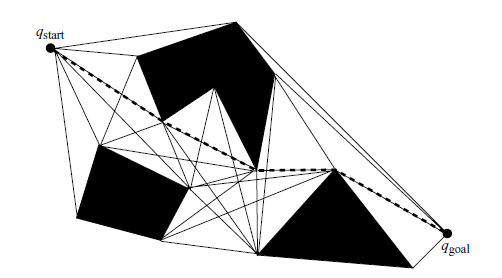
\includegraphics[width=0.8\textwidth]{images/Robot_Motion_Visibility_Graph.png}
	\caption{Von \cite[~S. 111]{Principles:05} \textit{Abb. 5.4} Die Linien begrenzen die Kanten des Sichtbarkeitsgraphen für die drei Hindernisse, die als gefüllte Polygone dargestellt sind. Die gepunktete Linie stellt den kürzesten Weg zwischen Start und Ziel dar.}
	\label{sec3a}
\end{figure}


%\section{Adjacency graph}
%%bbbb
%
%\section{Punktgraphen (Point Graphs)}
%
%
%\section{(Automatic Navmesh Calculation)}
%
%
%\subsection{Zerteilung des Navmesh (Navmesh Cutting)} 